\section{一元二次方程与二次函数的进一步讨论}
\subsection{一元二次方程与二次函数的基本知识}
\begin{know}
    \item\textbf{一元二次方程的求根公式}
    
    \item \textbf{二次函数}
    \item \textbf{根式的嵌套}
    \item \textbf{一元\(n\)次方程的Vieta定理}
\end{know}
\begin{definition}[一元\(n\)次方程]\label{def:一元n次方程}\index{一元\(n\)次方程}
    只有一个变量, 形如
    \begin{equation}
        a_nx^n+a_{n-1}x^{n-1}+\cdots+a_2x^2+a_1x+a_0=0\qquad a_n\neq 0
    \end{equation}
    称作一元\(n\)次方程. 其中\(n=2\)时就是我们常见的一元二次方程
    \begin{equation}
        ax^2+bx+c=0\qquad a\neq 0
    \end{equation}
\end{definition}

对于简单的一元二次方程, 都可以用配方法来求解, 
由此给出一元二次方程的求根公式. 
\begin{theorem}[一元二次方程的求根公式]
    对于形如\(ax^2+bx+c=0(a\neq0)\)的一元二次方程, 方程的两个根可以写作
    \begin{equation}
        x_{1,2}=\frac{-b\pm \sqrt{b^2-4ac}}{2a}.
    \end{equation}

    其中\begin{equation}
        \Delta=b^2-4ac
    \end{equation}
    称作一元二次方程的判别式, 当\(\Delta>0\)时, 方程有两个不等的实根；当\(\Delta=0\)时, 
    方程有两个相等的实根；当\(\Delta<0\)时, 方程没有实根, 而有一对共轭虚根. 
\end{theorem}
\begin{proof}
    方程两侧配方即可
    \begin{align*}
       ax^2+bx+c&=0\\
       x^2+\frac{b}{a}x&=-\frac{c}{a}\\
       x^2+\frac{b}{a}x+\frac{b^2}{4a^2}&=\frac{b^2}{4a^2}-\frac{c}{a}\\
       (x+\frac{b}{2a})^2&=\frac{b^2-4ac}{4a^2}\\
       x+\frac{b}{2a}&=\pm \sqrt{\frac{b^2-4ac}{4a^2}}\\
       x&=\frac{-b\pm \sqrt{b^2-4ac}}{2a}.
    \end{align*}

    
\end{proof}

不难发现, 解方程过程中存在着对\(\frac{b^2-4ac}{4a^2}\)开平方根的这一行为, 而分母\(4a^2\)恒正（注意我们提前预设了\(a\neq0\)）, 
当分子非负的时候才有实数解, 否则在实数范围内无意义. 

\begin{definition}[二次函数]\index{函数!二次函数}
    形如\(y=ax^2+bx+c\ (a\neq0)\)的函数称为二次函数. 这样的形式称为二次函数的一般式. 
\end{definition}

对于一般式的二次函数, 并不容易直接看出顶点、对称轴、单调区间这些信息. 
如果对一般式配方
\begin{align*}
    y&=ax^2+bx+c\\
    &=a(x^2+\frac{b}{a}x+\frac{c}{a})\\
    &=a(x^2+\frac{b}{a}x+\frac{b^2}{4a^2}+\frac{c}{a}-\frac{b^2}{4a^2})\\
    &=a(x+\frac{b}{2a})^2+\frac{4ac-b^2}{4a}
\end{align*}

由此引出二次函数的顶点式定义：
\begin{definition}
    称如同\(y=a(x-h)^2+k\)的形式为二次函数的顶点式. 
\end{definition}
对于一个二次函数而言, 通常是用平移的方法来研究的. 将\(y=ax^2\)
向右平移\(h\), 向上平移\(k\)后得到一个新的函数\(y=a(x-h)^2+k\). 
只要知道\(y=ax^2\)的各种性质, 那么\(y=ax^2+bx+c\)和\(y=a(x-h)^2+b\)的性质都迎刃而解了. 

\begin{character}
    对于二次函数\(y=ax^2+bx+c\)：

    顶点为\((-\frac{b}{2a},\frac{4ac-b^2}{4a})\), 对称轴为直线\(x=-\frac{b}{2a}\)；

    当\(a>0\)时, ；

    当\(a<0\)时, . 
\end{character}

\clearpage
\begin{example}[2025年天津卷15]\label{高考:2025年天津卷15}
    若\(a,b\in\mathbb{R}\),\(\forall x\in [-2,2]\), 均有
        \((2a+b)x^2+bx-a-1\leq 0\)恒成立, 求\(2a+b\)的最小值为\uline{\makebox[1.5cm]{}}.
\end{example}
\begin{jie}
    \begin{way1}
        希望$(2a+b)x^2+bx-a-1$在赋某值之后可以整理成\(2a+b\)的形式, 取 
        \(x=-\frac{1}{2}\), 得到\(\frac{1}{4}(2a+b)-\frac{1}{2}(2a+b)-1\leq 0\),
        即得到必要条件\(2a+b\geq -4\). 接下来只需验证可以取到\(-4\).

        由于二次函数最值应该在区间端点或对称轴处取得, 由上面观察可知应为\(-\frac{1}{2}\)是对称轴, 即 
        \[\left\{\begin{aligned}
            &2a+b=-4\\
            &\frac{b}{2(2a+b)}=-\frac{1}{2}
        \end{aligned}\right.\]
        解得\(b=-4,a=0\).此时原不等式化为
        \(-4x^2-4x-1=-(2x+1)^2\leq 0\), 这显然成立. 故\(2a+b\)的最小值为\(-4\). \qed
    \end{way1}
    \begin{way2}尝试将参数分离处理.
        设\(2a+b=t\), 则原不等式可以写为
        \(tx^2+(t-2a)x-a-1\leq 0\),
        即\[tx^2+tx\leq 2ax+a+1\]
        不等式左侧是二次函数, 右侧是恒过\((-\frac{1}{2},1)\)的直线.
        不等式成立的一个必要条件是左侧在\(-\frac{1}{2}\)的函数值小于等于\(1\),
        即\(\frac{1}{4}t-\frac{1}{2}t=-\frac{1}{4}t\leq 1\),  
        解得\(2a+b=t\geq -4\), 必要性验证同上.\qed
    \end{way2}
\end{jie}








%在这里讲一些根式的性质, 包括根号嵌套的分解
\clearpage
在初中学习过一元二次方程的韦达定理, 表述如下
\begin{theorem}[Vieta定理]\label{thm:Vieta定理}\index{Vieta定理}
    设\(x_1,x_2\)为一元二次方程\[ax^2+bx+c=0\]的两根, 则有根和系数的关系如下：
    \[
\left\{
\begin{array}{ccc}
  x_1 + x_2 & = &\displaystyle -\frac{b}{a} \\
  x_1 x_2   & = &\displaystyle \frac{c}{a}
\end{array}
\right.
\]%保证了居中
 
\end{theorem}
\begin{proof}
    \begin{way1}
        由求根公式
        \[x_1+x_2=\frac{-b+ \sqrt{b^2-4ac}}{2a}+\frac{-b-\sqrt{b^2-4ac}}{2a}=-\frac{b}{a}\]
        \[x_1x_2=\frac{-b+ \sqrt{b^2-4ac}}{2a}\frac{-b-\sqrt{b^2-4ac}}{2a}=\frac{(-b)^2-(b^2-4ac)}{4a}=\frac{c}{a}\]
    \end{way1}
    \begin{way2}

    \end{way2}

    \qed
\end{proof}

\begin{theorem}[Vieta定理]
    设\(x_1,\cdots,x_n\)为一元\(n\)次方程
    \begin{equation}
        a_nx^n+\cdots+a_1x+a_0=0\qquad(a_n\neq0)
    \end{equation}的\(n\)个根, 则由根和系数的关系如下：
    \[
        \left\{
        \begin{array}{ccc}
          \displaystyle\sum_{i=1}^{n}x_i& = &-\dfrac{a_{n-1}}{a_n} \\
          \displaystyle\sum_{i\neq j}x_ix_j   & = &\dfrac{a_{n-2}}{a_n}\\
          \displaystyle\sum_{i\neq j\neq j}x_ix_jx_k&=&-\dfrac{a_{n-3}}{a_n}\\
          \cdots&\quad&\cdots\\
          \displaystyle\prod_{i=1}^{n}x_i&=&(-1)^n\dfrac{a_0}{a_n} 
        \end{array}
        \right.
        \]






\end{theorem}
\clearpage
\subsection{根的分布}
\begin{know}
    \item \textbf{一元二次方程根的分布}
\end{know}
\begin{theorem}[介值性]\label{thm:介值性}
    \ 

    若$f(x)$连续, 不妨设$f(a)<f(b)$, $\forall \mu \in(f(a),f(b))$, 
    则$\xi \in [a,b]$,使得$f(\xi)=\mu$.

    特别地, 当$\mu=0$时, 有根的存在性原理. 

    若$f(x)$连续, 且$f(a)f(b)<0$, 则至少存在一点$x_0 \in (a,b)$,使得$f(x_0)=0$. 
    换言之方程$f(x)=0$在$(a,b)$上至少有一个根. 
\end{theorem}
\begin{zhu}
    这个定理的证明高中阶段无法完成, 尽管它是如此符合数学直觉. 
\end{zhu}

这节就是在定理\ref{thm:介值性}的基础上, 限定根存在的条件, 最终目标是确定某一个参数的取值范围. 

而我们的武器就是图像, 先根据题目画出草图, 再对函数加以限制. 

比如开口方向（二次项系数$a$）, 对称轴（$-\frac{b}{2a}$）, 
根的数量（$\Delta=b^2-4ac$）, 根的具体区间（特殊点的正负）. 

我们接下来通过一个具体的例子来说明具体是如何操作的. 
\begin{example}\label{example 2.3.1}
    \[f(x)=8x^2-(m-1)x+(m-7)\]

$(1)x_1>1$,$x_2>1$

$(2)x_1>2$,$x_2<2$

$(3)x_1,x_2\in (0,2)$

$(4)\text{两根异号且}|x_1|<1,|x_2|<1$
\end{example}
\begin{analyse}
此题的二次项系数已经固定为正了, 我们只要讨论其他的三件事即可. 先根据题目画出草图. 
注意这个草图也是有讲究的, 你需要在草图上清晰地展示出来根所在的位置. 
\end{analyse}

        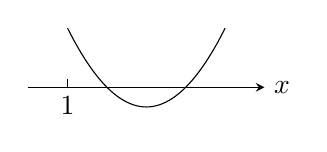
\begin{tikzpicture}[>=stealth]
        \draw [->](0.5,0)--(3.5,0)node[right]{$x$};%分号不能省略,node命令是用来标记的
        \foreach \x in {1}%用来在x轴上标数
        {
            \draw (\x,0)node[below]{$\x$}--(\x,0.1);
        }
        \draw[domain=1:3,smooth]%domain定义域
        plot(\x,{\x*\x-4*\x+3.75});
        \end{tikzpicture}
        \hspace{2.5em}
        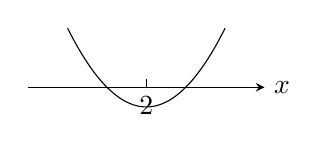
\begin{tikzpicture}[>=stealth]
        \draw [->](0.5,0)--(3.5,0)node[right]{$x$};
        \foreach \x in {2}
        {
         \draw (\x,0)node[below]{$\x$}--(\x,0.1);
        }
        \draw[domain=1:3,smooth]
        plot(\x,{\x*\x-4*\x+3.75});
        \end{tikzpicture} 
        
        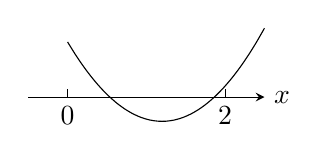
\begin{tikzpicture}[>=stealth]
        \draw [->](-0.5,0)--(2.5,0)node[right]{$x$};
        \foreach \x in {0,2}
        {
        \draw (\x,0)node[below]{$\x$}--(\x,0.1);
        }
        \draw[domain=0:2.5,smooth]
        plot(\x,{0.7*(\x*\x-2.4*\x+1)});
        \end{tikzpicture} 
        \hspace{2.5em}
        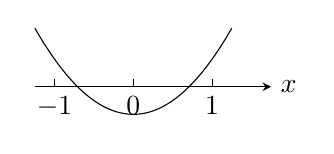
\begin{tikzpicture}[>=stealth]
        \draw [->](-1.25,0)--(1.75,0)node[right]{$x$};
        \foreach \x in {-1,0,1}
        {
            \draw (\x,0)node[below]{$\x$}--(\x,0.1);
        }
        \draw[domain=-1.25:1.25,smooth]
        plot(\x,{0.7*(\x*\x-0.5)});
        \end{tikzpicture}   


\begin{jie}
根据我们画的草图, 我们逐个判断判别式, 对称轴, 特殊点的正负这些要素. （二次项系数这里已经确定了）

其中\[\Delta=[-(m-1)]^2-4\times8(m-7)=(m-1)^2-32(m-7)=m^2-34m+225\]
\[\text{对称轴为直线}x=-\frac{-(m-1)}{16}=\frac{m-1}{16}\]

$(1)$ 
\[  
    \left\{
    \begin{lgathered}
    \Delta\geq 0\\
    \frac{m-1}{16}>1\\
    f(1)>0
    \end{lgathered}
    \right.
\]

解得$m \in [25,+\infty)$

$(2)$
\[  
    \left\{
    \begin{lgathered}
    \Delta > 0\\
    f(2)<0
    \end{lgathered}
    \right.
\]

解得$m \in (27,+\infty)$

$(3)$
\[  
    \left\{
    \begin{lgathered}
    \Delta \geq 0\\
    0<\frac{m-1}{16}<2\\
    f(2)>0\\
    f(0)>0
    \end{lgathered}
    \right.
\]

解得$m \in (7,9]\cup[25,27)$

$(4)$
\[  
    \left\{
    \begin{lgathered}
    \Delta > 0\\
    -1<\frac{m-1}{16}<1\\
    f(-1)>0\\
    f(0)<0\\
    f(1)>0
    \end{lgathered}
    \right.
\]

解得$m \in (0,7)$
\end{jie}
\begin{att}
这是讲义中第一次出现列不等式组, 解不等式组的问题. 在这时要尤其注意在把条件翻译成不等式的时候, 究竟能不能取等号. 

以例$\ref*{example 2.3.1}$中的$\Delta$为例, 其中$\Delta$究竟是大于$0$还是大于等于$0$就很有说法. 我们在初中的时候应该强调过, 
二次方程的$\Delta=0$是指方程有两个相等的实根（而非一个实根）, $\Delta>0$是指方程有两个不等的实根. 

现在你能够理解为什么$(1)(3)$带等号, 而$(2)(4)$不带等号了吗？

另外, 你知道上述过程中哪里使用了定理\ref{thm:介值性}吗？
\end{att}

有了例$\ref*{example 2.3.1}$, 现在你可以尝试着自己总结一下关于根的分布的各种情况了. 

对于函数\[f(x)=ax^2+bx+c\quad(a\neq0)\]
\begin{enumerate}
    \item 两根与某一个数$m$比较. 
    
    即两根都大于$m$, 两根都小于$m$, 两根一个大于一个小于$m$. 

    \item 两根与一个区间$(m,n)$端点的比较. 
    
    这个情况略复杂. 光是根与区间关系就有6种. 6种可以看做有3类, 区间内有0个, 1个, 2个根. 

    区间内有0个根中的两种情况, 两根在都区间左侧和两根都在区间右侧, 是可以看做是情况1. 
    另外一种是两根在区间外, 但一根在区间左侧, 一根在区间右侧. 

    区间外的根讨论完了, 接下来是区间内的根. 
    区间内有1个根是两种情况（另一根在区间左侧或在区间右侧）, 最后是区间内有2个根. 
    \item 一根在$(m,n)$内, 另一根在$(p,q)$内. 
\end{enumerate}

\begin{zhu}
    针对“方程有且仅有一根在区间内”的情况, 有时候会把$\Delta=0$的情况也放进去, 
    这并非是数学概念上的不严谨. 有时候我们需要就解出来一个数, 两个重根这时候确实是一个数. 
\end{zhu}

当然这样的题目除了在高一练习的时候往往不会单独出现, 更多时候是某个题目经过若干变形, 最后转化为根的分布问题. 
\begin{exercise}
    已知函数\[f(x)=2ax^2+2x-3-a\quad(a\in \mathbb{R} )\]

    若函数$y=f(x)$在区间$[-1,1]$上有根, 求$a$的取值范围. 
\end{exercise}
\begin{exercise}
    二次方程\[(m-1)x^2+(3m+4)x+(m+1)=0 \]

    的两根都在$(-1,1)$内, 求$m$的取值范围. 
\end{exercise}
\begin{exercise}
    二次函数$f(x)=px^2+qx+r$中实数$p,q,r$满足
    \[\frac{p}{m+2}+\frac{q}{m+1}+\frac{r}{m}=0\]

    其中$m>0$, 求证：

    $(1)$\[pf(\frac{m}{m+1})<0\]

    $(2)$方程$f(x)=0$在$(0,1)$上总有解. 
\end{exercise}










\clearpage
\subsection{在区间内的最值}
\begin{know}
    \item \textbf{二次函数在区间内的最值}
\end{know}
在初中中我们学过, 对于开口向上的抛物线, 在对称轴处取得最小值；对于开口向下的抛物线, 在对称轴处取得最大值.
但是如果自变量的取值不是全体实数, 而是被限制在了某一个区间内呢？这时候就需要用到这节的分类讨论了.

我们讨论是的时候也应该有对应的主线. 先讨论二次项次数：是不是二次函数, 开口向上还是向下？
接下来就是对称轴, 与区间和区间中点的关系.当然这样干巴地讲解肯定意义不大, 我们来两道经典的例题.
\begin{example}
    求$f(x)=mx^2+6x-2$在$[1,2]$上的最大值$g(m)$.
\end{example}
\begin{analyse}
\end{analyse}
\begin{jie}以$m$的大小为线索讨论

$(1)$$m=0$, $f(x)$为一次函数, $f(x)_{max}=f(x)=10$

$(2)$$m>0$, 讨论对称轴与区间的关系, 此处$-\frac{3}{m}<0$, 可以一定程度上化简问题. 
画图可知, $f(x)_{max}=f(2)=4m+10$

$(3)$$m<0$,画图可知分为三种情况

\ding{172}$-\frac{3}{m} \in (0,1)$, 即$m \in (-\infty,-3)$, 
$f(x)_{max}=f(1)=m+4$

\ding{173}$-\frac{3}{m} \in [1,2]$, 即$m \in [-3,-1.5]$, 
$f(x)_{max}=f(-\frac{3}{m})=-2-\frac{9}{m}$

\ding{174}$-\frac{3}{m}>2$, 即$m \in (-1.5,0)$, 
$f(x)_{max}=f(2)=4m+10$

综上所述, 
\begin{equation}\notag
    g(m)=f(x)_{max}=\left\{
        \begin{aligned}
        4m+10    \qquad\    m \in (0,+\infty)\\
        10       \qquad\qquad\qquad\qquad   m=0\\
        4m+10    \qquad\    m \in (-1.5,0)\\
        -2-\frac{9}{m}   \qquad   m \in [-3,-1.5]\\
        m+4      \qquad\quad   m \in (-\infty,-3)\\
        \end{aligned}
        \right.
\end{equation}
    
不难发现, 前三种情况可以合并, 即写作
\begin{equation}\notag
    g(m)=f(x)_{max}=\left\{
        \begin{aligned}
        4m+10    \qquad\    m \in (-1.5,+\infty)\\
        -2-\frac{9}{m}    \quad\qquad  m \in [-3,-1.5]\\
        m+4      \qquad\qquad   m \in (-\infty,-3)\\
        \end{aligned}
        \right.
\end{equation}
\end{jie}
\begin{comment}
若题目指定了函数类型, 比如明确说明$f(x)$是二次函数, 
则意味着$m\neq0$, 无需考虑$m=0$的情况, 答案中也务必不要写$m=0$.
\end{comment}

上例是典型的“动轴定区间”, 这可以很自然地反过来, 即“定轴动区间”.

\begin{example}
    函数$f(x)=x^2-2x+2$在闭区间$[t,t+1]$上最小值记作$g(t)$,求$g(t)$.
\end{example}
\begin{jie}
    
\end{jie}
\clearpage